%%
%% This is file `sample-sigconf.tex',
%% generated with the docstrip utility.
%%
%% The original source files were:
%%
%% samples.dtx  (with options: `all,proceedings,bibtex,sigconf')
%% 
%% IMPORTANT NOTICE:
%% 
%% For the copyright see the source file.
%% 
%% Any modified versions of this file must be renamed
%% with new filenames distinct from sample-sigconf.tex.
%% 
%% For distribution of the original source see the terms
%% for copying and modification in the file samples.dtx.
%% 
%% This generated file may be distributed as long as the
%% original source files, as listed above, are part of the
%% same distribution. (The sources need not necessarily be
%% in the same archive or directory.)
%%
%%
%% Commands for TeXCount
%TC:macro \cite [option:text,text]
%TC:macro \citep [option:text,text]
%TC:macro \citet [option:text,text]
%TC:envir table 0 1
%TC:envir table* 0 1
%TC:envir tabular [ignore] word
%TC:envir displaymath 0 word
%TC:envir math 0 word
%TC:envir comment 0 0
%%
%%
%% The first command in your LaTeX source must be the \documentclass
%% command.
%%
%% For submission and review of your manuscript please change the
%% command to \documentclass[manuscript, screen, review]{acmart}.
%%
%% When submitting camera ready or to TAPS, please change the command
%% to \documentclass[sigconf]{acmart} or whichever template is required
%% for your publication.
%%
%%
\documentclass[sigconf]{acmart}

%%
%% \BibTeX command to typeset BibTeX logo in the docs
\AtBeginDocument{%
  \providecommand\BibTeX{{%
    Bib\TeX}}}

%% Rights management information.  This information is sent to you
%% when you complete the rights form.  These commands have SAMPLE
%% values in them; it is your responsibility as an author to replace
%% the commands and values with those provided to you when you
%% complete the rights form.
\setcopyright{acmlicensed}
\copyrightyear{2024}
\acmYear{2024}
\acmDOI{XXXXXXX.XXXXXXX}

%% These commands are for a PROCEEDINGS abstract or paper.
\acmConference[Conference acronym 'XX]{Make sure to enter the correct
  conference title from your rights confirmation emai}{June 03--05,
  2018}{Woodstock, NY}
%%
%%  Uncomment \acmBooktitle if the title of the proceedings is different
%%  from ``Proceedings of ...''!
%%
%%\acmBooktitle{Woodstock '18: ACM Symposium on Neural Gaze Detection,
%%  June 03--05, 2018, Woodstock, NY}
\acmISBN{978-1-4503-XXXX-X/18/06}


%%
%% Submission ID.
%% Use this when submitting an article to a sponsored event. You'll
%% receive a unique submission ID from the organizers
%% of the event, and this ID should be used as the parameter to this command.
%%\acmSubmissionID{123-A56-BU3}

%%
%% For managing citations, it is recommended to use bibliography
%% files in BibTeX format.
%%
%% You can then either use BibTeX with the ACM-Reference-Format style,
%% or BibLaTeX with the acmnumeric or acmauthoryear sytles, that include
%% support for advanced citation of software artefact from the
%% biblatex-software package, also separately available on CTAN.
%%
%% Look at the sample-*-biblatex.tex files for templates showcasing
%% the biblatex styles.
%%

%%
%% The majority of ACM publications use numbered citations and
%% references.  The command \citestyle{authoryear} switches to the
%% "author year" style.
%%
%% If you are preparing content for an event
%% sponsored by ACM SIGGRAPH, you must use the "author year" style of
%% citations and references.
%% Uncommenting
%% the next command will enable that style.
%%\citestyle{acmauthoryear}


%%
%% end of the preamble, start of the body of the document source.
\begin{document}

%%
%% The "title" command has an optional parameter,
%% allowing the author to define a "short title" to be used in page headers.
\title{Ontology Construction for Database Statistics in Preparation for Learning Integration}

%%
%% The "author" command and its associated commands are used to define
%% the authors and their affiliations.
%% Of note is the shared affiliation of the first two authors, and the
%% "authornote" and "authornotemark" commands
%% used to denote shared contribution to the research.
\author{Leo Scott Fitzsimmons}
\affiliation{%
  \institution{Charleston Southern University}
  \city{North Charleston}
  \state{SC}
  \country{USA}
}
\email{lsfitzsimmons@csustudent.net}

\author{Songhui Yue}
\affiliation{%
	\institution{Charleston Southern University}
	\city{North Charleston}
	\state{SC}
	\country{USA}
}
\email{syue@csuniv.edu}

\author{Sean Hayes}
\affiliation{%
	\institution{Charleston Southern University}
	\city{North Charleston}
	\state{SC}
	\country{USA}
}
\email{shayes@csuniv.edu}
	
\author{Valerie Session}
\affiliation{%
	\institution{Charleston Southern University}
	\city{North Charleston}
	\state{SC}
	\country{USA}
}
\email{vsessions@csuniv.edu}


%%
%% By default, the full list of authors will be used in the page
%% headers. Often, this list is too long, and will overlap
%% other information printed in the page headers. This command allows
%% the author to define a more concise list
%% of authors' names for this purpose.
\renewcommand{\shortauthors}{Trovato et al.}

%%
%% The abstract is a short summary of the work to be presented in the
%% article.
\begin{abstract}
Ideally, data-focused researchers and database administrators should easily reference statistics and other relevant metadata about their databases, but statistical information often requires additional skills and effort to be manually extracted into an easily consumable, understandable format. This research aims at an automatic methodology for constructing and visualizing an ontology for database statistics. The collected metadata and statistics are transformed and presented visually alongside corresponding objects in a database ontology graph. Statistics are included to enrich the ontology graph for increasing researcher knowledge and may assist in learning integration tasks such as ontology simplification, decision-making for database design and optimization, and ingestion by other artificial intelligence (AI) processes. The results of this research consist of a methodology for complementing database ontology graphs with statistics details, a candidate model for database statistics ontology, and use cases of potential learning integrations.
\end{abstract}

%%
%% The code below is generated by the tool at http://dl.acm.org/ccs.cfm.
%% Please copy and paste the code instead of the example below.
%%
\begin{CCSXML}
	<ccs2012>
	<concept>
	<concept_id>10002951.10002952.10003219.10003215</concept_id>
	<concept_desc>Information systems~Extraction, transformation and loading</concept_desc>
	<concept_significance>500</concept_significance>
	</concept>
	<concept>
	<concept_id>10002951.10003317.10003318.10011147</concept_id>
	<concept_desc>Information systems~Ontologies</concept_desc>
	<concept_significance>500</concept_significance>
	</concept>
	<concept>
	<concept_id>10002951.10003317.10003347.10011712</concept_id>
	<concept_desc>Information systems~Business intelligence</concept_desc>
	<concept_significance>300</concept_significance>
	</concept>
	</ccs2012>
\end{CCSXML}

\ccsdesc[500]{Information systems~Extraction, transformation and loading}
\ccsdesc[500]{Information systems~Ontologies}
\ccsdesc[300]{Information systems~Business intelligence}

%%
%% Keywords. The author(s) should pick words that accurately describe
%% the work being presented. Separate the keywords with commas.
\keywords{Ontology, Database, Statistics, Interoperability, Visualization}
%% A "teaser" image appears between the author and affiliation
%% information and the body of the document, and typically spans the
%% page.

%%
%% This command processes the author and affiliation and title
%% information and builds the first part of the formatted document.
\maketitle

\section{Introduction}
An ontology is a set of concepts and categories within a subject area or domain that defines their properties and the relationships between them. It forms the scaffolding that establishes standard terms, labels, and relationships, creating a common language for both structured and unstructured data \cite{gruber1993ontology, chari2020explanation}. Ontology allows for the processing and understanding of data upon the defined, common categorization of data and relationships. \cite{yue2023csm}. One of the major objectives of ontology is to make knowledge in a domain computationally useful \cite{tudorache2020ontology}. For heterogeneous systems, it provides a common language by which disparate systems can communicate \cite{fraga2020ontology, yue2023csm}. For AI systems, it gives context to data and enables AI to “decide” based on content and relationship. Ontology graphs are a way to visually represent an ontology and increase learning and understanding of a domain. They provide a visual representation of relationships between classes, attributes, and properties \cite{gutierrez2018knowledge, yue2021applying}.

A multitude of resources (vendor documentation, subject matter expert (SME) articles, and posts \cite{RWesta, RWestb, RWestc}) address RDBMS statistics maintenance (specifically Microsoft SQL Server© --or the rest of the document, referred to as “SQL Server”) and how the query optimizer uses statistics and histograms. The vast majority of the writings are functional and pragmatic, addressing how to solve issues related to performance. Academic work related to database statistics and histograms is sparse; the limited information is curious because there are intricacies and subtleties to statistics updates and histograms, which make the query optimizer choose questionable plans that lead to poor and often unpredictable performance. Most efforts to resolve these issues are labeled and resolved as “statistics maintenance” problems and do not go much further. Furthermore, histogram data, primarily used
by the query optimizer, are available to the analyst and have the potential for analysis and mining, but querying and presenting these data can be somewhat cumbersome and have a less-than-desirable default format.

The scarcity of information/research regarding database statistics—specifically index utilization, column statistics, and histograms—and lack of deep study/mining into the same motivates this research. This effort first produces a statistics ontology to establish a standard ontology for database statistics based on the subject matter knowledge of the RDBMS. It is intended for the ontology to define a domain and assist in making the statistics data “computationally useful.” The ontology shows database statistics as they exist at different levels, taking opportunities to aggregate characteristics or flag important aspects. Next, with the resultant ontology in mind, a semi-automated process has been created and executed. The process produces two ontology graphs: an ontology graph centered on column statistics and an ontology graph based on index utilization. This transformation effort also produces enriching data in a supporting Hypertext Markup Language (HTML) document. Figure \ref{overview} below summarizes the full objective. The resultant ontology helps promote learning and establish a framework from which data can potentially be formatted for use by machine learning/AI.

\begin{figure}[h]
	\centering
	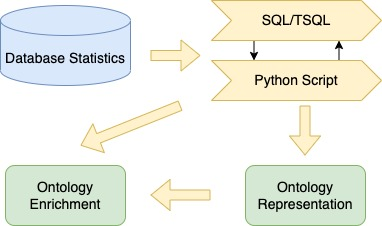
\includegraphics[width=0.8\linewidth]{db-statistics-ontology}
	\caption{An Overview of the Study.}
	\label{overview}
\end{figure}

This work contributes to database statistics learning, reinforcing metadata concepts by visually organizing and representing statistics on appropriate object (table, index, column) levels. This work also contributes to statistics ontology (and, more specifically, database-related statistics) as it can be a starting point for future work regarding database statistics modeling and mining opportunities using machine learning or other AI methods.

\section{Related Work}
There is a significant amount of research regarding ontology (in the scope of computer science) and the automatic/semiautomatic creation of ontology, especially as extracted from a relational database; the related works highlight many of these efforts, to include Protégé, RDB2OWL, and Mapping of Relational Schema \cite{christian2017mapping}. Deeper or specific understanding and learning are achieved by incorporating “enriching” data into the ontology, added in from an external source. Examples of automatic/semiautomatic ontology enrichment are the works by Booshehri and Luksch \cite{booshehri2015ontology} and Rajput and Gurulingappa \cite{rajput2013semi}.

Creating an ontology can be very manually intensive and often requires domain expert involvement, so a great deal of research and effort has been given to automate the task of ontology creation. There are several research documents that summarize ontology approaches; for example, the approach in \cite{christian2017mapping} is very similar to this research, with at least the major difference of the RDBMS (Oracle) platform. The research conducted in the work of Loudi et al. \cite{louhdi2013hybrid} is also similar, using MySQL RDBMS. Būmans and Čerāns \cite{bumans2018rdb2owl} outline a process to map the database entities to Web Ontology Language (OWL) and includes a schema that may be used and/or improved. In these cases, the ontology was focused on a user schema/data, not statistics, and not toward a standardization or extraction of statistical metadata. Issues common to building an ontology are the following:
\begin{itemize}
\item Domain experts needed for validation.
\item Objects such as views may not translate into ontology, or important facts or relationships are sometimes missed.
\item Ontology creation is dependent on the domain and the purpose of the ontology.
\end{itemize}
	
Database statistics, particularly in SQL Server, have been the subject of numerous white papers, conference sessions, blogs, and “best practices” lists. More specifically, the attention is more so on the maintenance of statistics due to their importance in accurately representing the actual data. Likewise, the primary purpose of the histogram is internal use; the query optimizer uses a column’s histogram to help estimate the number of rows a query will return. It is speculated that due to their functional nature and common perception of “internal use only” by the RDBMS, there is very little if any, academic-level research on column statistics and histograms. The work by Lee et al. \cite{lee2016operator} addressed the operation of SQL Server Live Query Statistics feature, but no other scholarly works have addressed or capitalized on the internal collections or analysis of statistics metadata.

\section{Motivation and Use Cases}
Numerous ontology-from-relational-database generation efforts are successful in converting data definition language (DDL) output into OWL format. It is common to have external enriching data to help with context and understanding, and ontology is a “knowledge scaffolding” upon which AI can be built. A relational database, due to its structure and data organization, provides an effective platform not only to extract the metadata but to work with business data as well. With these characteristics and ideas in mind, the intended objectives of the research effort are listed below and explained with use cases in the subsections:

\begin{itemize}
	\item Produce a database statistics ontology
	\item Produce statistics-centric ontology graphs with enriched data resources
	\item Prepare for data mining opportunities
\end{itemize}

\subsection{Motivation I: Produce a Database Statistics Ontology}
Ontology, by definition, specifies a common vocabulary for a domain or subject, and
from this common vocabulary, information can be exchanged between heterogeneous systems. When using ontology, the goal is to use semantic-level representation, meaning it is formal and independent of modeling or implementation strategies \cite{gruber}. In order to better understand database statistics and their importance when evaluating a database ontology, this research is to produce a database statistics ontology in the XML format and displayed as an ontology graph (via WebVOWL) and regular diagram.

\subsection{Motivation 2: Produce an Ontology Graph With Enriched Data}
An analysis of the data themselves is typically used to improve the accuracy and
understanding of an ontology, but collecting information about the data in a useful manner can be cumbersome and time consuming. There may not be a full replacement for independently evaluating column data and table usage manually, and it is a time and resource-intensive step. Furthermore, the ontology creation process may collapse or process out important data features. Whereas enrichment is commonly from outside source—such as the Wikipedia \cite{tramontana2022ontology} and DBpedia \cite{booshehri2015ontology} examples—this research proposes the source of enrichment to be sourced from the data automatically and semi-automatically collected and formatted by the RDBMS. It is intended to identify and then effectively display meaningful statistical characteristics in the ontology graph for manual or automatic assessment. 

\subsection{Motivation 3: Prepare for Data Mining Opportunities}
Although some rollup or generic statistics such as “Number of Tables” or “Is Used in
Index” are helpful for research and design purposes, the primary purpose of column statistics and the column histogram is for internal use by the query optimizer to estimate query plans. Column statistics can be viewed with TSQL in SSMS, and histogram data can be viewed via SSMS (see Figure 3) as well as by utilizing TSQL and built-in stored procedures. Histogram formatting is tedious to work with, and the gathering of its data is multi-step. Manual or programmatic evaluation of a histogram may show data skew or other noteworthy distributions of data, but this method of use is minor at best. Database statistics and histograms are not commonly used outside
of the query optimizer, so it is rather novel territory to utilize the information in this way. With the overwhelming amount of information and disparate statistics formats, an ontology would provide the structure needed to best organize the data and prepare it in a format that could be consumed by a processing program (perhaps AI), that could mine the information. 

\subsection{Use Case 1: Establish and increase knowledge of a domain}
As previously described, an ontology defines a domain with common terms to be used by heterogeneous systems. Whether ontologies are created manually or automatically generated, they are refined by subject matter experts (SME) (The author does not claim to be an SME for database statistics, but based on real-world experience). Creating a database statistics ontology aids in the understanding of statistics (what information is available at what level) and establishes the framework for creating database statistics-centric ontologies that may be used to describe a database on a statistical level or be used to compare statistics between systems.
Example: A junior database administrator (DBA) or analyst is tasked with comparing schemas from different databases. They haven’t worked with database statistics and therefore unfamiliar with what is collected or even available. Without the statistics knowledge, they resort to selecting counts from every table, researching columns for distinct values. And maybe even attempting to collect information with custom processes. If the analyst referenced the database statistics ontology, they would better understand what is already available and at what object level.

\subsection{Use Case 2: Importance of relationships, tables, and indexes}
Ontology visual tools or generating tools have the ability to “collapse”, essentially pruning off attributes or combining classes. The pruning/collapsing may be based on degree or “connectedness” to other classes or attributes that may be pruned off and deemed unnecessary to the ontology. Manual intervention can correct such exclusions, but it requires expert knowledge of the subject matter. There are also techniques to analyze the data programmatically to find possible missing elements, which may require additional passes for the needed analysis. The proposed work relies on statistical data already collected by the RDBMS. It will display index and table usage statistics inline in the ontology graph and amplify information in HTML that can assist in the evaluation of the importance of the relationship.

Example: An ontology is created from a Human Resources-related schema. Based on its processing rules, it prunes off a relationship between two tables that was represented by a foreign key (which also has an index). The analysis of this research shows that the index was used 98\% of the time when the table was accessed. In this case, the ontology creation process deems the relationship unimportant, whereas the enriched data may indicate otherwise. Similarly, the proposed study will produce data that will help compare the “importance” of indexes and tables to each other overall.

\subsection{Use Case 3: Preparation for Mining}
Poor maintenance of statistics leads to inaccurate statistics, and inaccurate statistics lead to bad execution plans and poor and often inefficient query performance. Statistics sample size and frequency of statistics updates play major roles in statistics accuracy. A sample size of statistics updates can be especially inaccurate due to RDBMS row count thresholds and whether or not automatic statistics updates are enabled. Likewise, the update frequency is troublesome because the internal thresholds set for automatic statistics updates are often not triggered early enough to avoid bad execution plan estimates. There is a multitude of strategies and scripts to get statistics to behave consistently, and their use is viewed as functional, not complementary to database/data work. Statistics information is used mainly for troubleshooting when statistics are suspected to be contributing to poor query performance. With multiple variables such as formatting, timing of automatic and manual statistics updates, percent of rows sampled for manual statistics updates, poor percentage of rows sampled on automatic updates, and varying triggering levels of row modifications based on row counts, how can all the relevant data be collected and formatted for analysis? How can information from a histogram, in its current format, be analyzed? By using an ontology, the data can be formatted and prepared for ingestion by a system trained to know what to do with the data.

\section{Methodology}

\subsection{Modeling}
Figure \ref{statistics-class-diagram} presents a class diagram of the db statistics that we are concerning with. We would like to embed those data into the generated ontology, as an enrichment. as a meaningful enrichment. To achieve this, we will build an ontology based on the model in the figure itself. Thus, for each type of the databases, we can explore various ways and concerns to enrich those data, becuase for different domain of knowledge, it might need different business logic to concern with so that different aspects in the statistics will be emphasized. That is for future work.

\subsection{Data Processing}

\subsubsection{Part I—Create a Database Statistics Ontology (Column and Index)}
Based on subject matter expert experience and knowledge of the RDBMS (specifically
SQL Server), an ontology for database statistics was created and revised first via UML diagram and then converted manually to XML. The OWL language was used to represent the database statistics ontology as an ontology graph. A text editor was first used to compose OWL and XML code. Next, the web-based utility WebVOWL was utilized to validate and visually display the resultant ontology graph. The ontology created is the framework for the creation of ontology graphs for a given target schema. 

\begin{figure}[h]
	\centering
	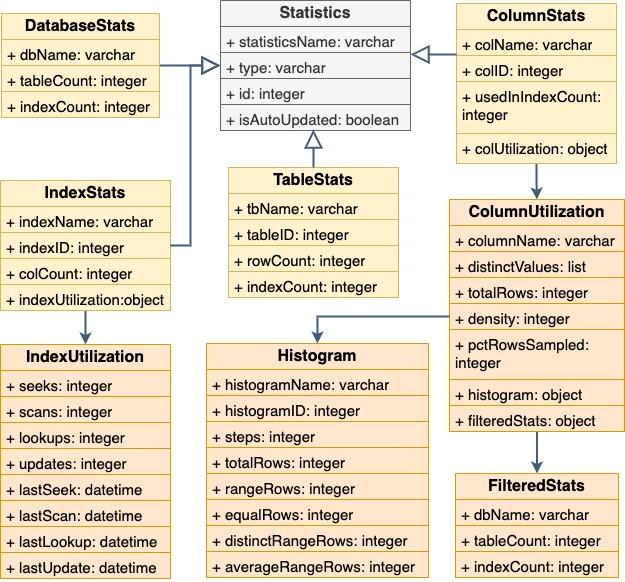
\includegraphics[width=\linewidth]{uml-db-statistic}
	\caption{A UML Class Diagram of Database Statistics Ontology.}
	\label{statistics-class-diagram}
\end{figure}

\subsubsection{Part II—Generate Column and Index Ontology Graphs With Enriched Data}
Noy and McGuinness \cite{noy2001ontology} suggested three fundamental rules for ontology creation, one which is “There is no one correct way to model a domain— there are always viable alternatives.” As such, the proposed methodology is presented. It consists of a collection of tables in a schema isolated from the target schema in the RDBMS, scripts to collect and transform the data, and a Python script to construct a Resource Description Framework Schema (RDF) OWL formatted file and an HTML file. The final step is visual representation and analysis using WebVOWL. Figure 6 represents the high-level workflow.

\subsubsection{Part III—Extract Metadata to OWL/XML for Overall/Column Statistics Ontology}
Using Python scripts and JDBC connections to the SQL Server instance, the OntologyEngine tables were sourced to wrap/transform data into OWL format and write to XML file. This extraction included all tables, columns, relationships, and enriching data at the appropriate object level. Additional logic for data mining may take place for additional insights.

\subsubsection{Part IV—Visualize and Evaluate}
The WebVOWL utility at https://service.tib.eu/webvowl/ is sourced, and the created XML is used as input. The ontology graph is checked for accuracy, and the enriching data noted. Functions such as collapse and re-evaluate will be used as needed.

\subsection{Plan for Experimentation and Evaluation}
The objective is to build a semi-automated way to construct ontology for DB statistics, as a priliminary work for a full automated method. Also, according to the use cases, we will develop detailed use cases in order to demonstrate the neccesity of it, to demonstrate the learning integration with AI and business intelligence. For builidng the overall workflow, the test will contain the following parts.

\begin{itemize}
\item Evaluation/Review of the Statistics Ontology Setup and Execution
\item Base Data Collected, No Enriching Data for Column Statistics Simulated.
\item Evaluation of Ontology Graph Produced in Test 2, Allowing Enriched Data.
\item Collection of Index Utilization Statistics, Generation of HTML Enriching Data.
\item Generation of Index-Oriented Statistics Ontology on Target Schema.
\item Evaluation of the Accuracy and Completeness.
\end{itemize}

\section{Conclusion / Future Work}
This research produce the intended ontology for database statistics in XML format,
using OWL, and display via WebVOWL. The ontology is used as a framework
to creating a process that collect, transform, and extract data to XML files, producing statistics-centric ontologies. The generated ontologies included graphs of column-based statistics, index utilization statistics, and supporting HTML documents with enriching data. Further efforts may work toward improving and formalizing the ontology such that it can be used practically as a standard resource ontology. Other ontologies exist as standard and are referenced (there were several used by the generated ontologies in this research). After refinement and formalization, the ontology could be an official reference; including additional subject matter experts to review may give additional insight and refinement. Next, continuing to pursue efforts with machine learning/AI by creating an application to extract/consume/use the data is highly recommended, possibly in artificial intelligence or other technology for decisioning. 

Use of AI/ML technologies to analyze the statistics and identify data skew, troublesome statistics, or inefficient indexes may lead to better insights and database/query engine improvement. AI/ML most likely has more logic, processing, and learning capabilities than current methods and techniques; processes could be developed for deeper analysis and mining of the histograms and index utilization. Third, advancing research with current RDBMS metadata for additional opportunities and information may enhance the ontology or offer opportunities to roll up information. Finally, research may move one step further with standardization of ontology by expanding to other types of database management system (DBMS) platforms, such as NoSQL, or Graph DB. 

%%
%% The acknowledgments section is defined using the "acks" environment
%% (and NOT an unnumbered section). This ensures the proper
%% identification of the section in the article metadata, and the
%% consistent spelling of the heading.

%%
%% The next two lines define the bibliography style to be used, and
%% the bibliography file.
\bibliographystyle{ACM-Reference-Format}
\bibliography{sample-base}


%%
%% If your work has an appendix, this is the place to put it.

\end{document}
\endinput
%%
%% End of file `sample-sigconf.tex'.
